% Se usa la clase TesisUNI que es basada en la clase book
% Requiere que en la carpeta raíz se encuentre el archivo TesisUNI.cls
\documentclass[11pt,a4paper,oneside,english,spanish]{TesisUNI}

% PREAMBULO: configuración general
%Encoding
\usepackage[utf8]{inputenc} %entrada %https://tex.stackexchange.com/questions/13067/utf8x-vs-utf8-inputenc
\usepackage[T1]{fontenc} %salida

%Manejo de referencias en estilo APA
\usepackage[natbibapa]{apacite} %Agregar formato de citación APA
\bibliographystyle{apacite} %Puede definirse al cargar la lista de referencias
\setlength{\bibsep}{5pt plus 0.3ex} %Espaciamiento en la bibliografía

\usepackage[spanish, es-tabla]{babel} % es-tabla reemplaza "cuadro" por "tabla"
\usepackage{layouts} %Saber ancho de hoja
%\usepackage{fontspec}

\usepackage{mathptmx}
\usepackage{amssymb} %Símbolos matemáticos
\usepackage[mathbf=sym]{unicode-math} % Mantener fuentes matemáticas

\usepackage{graphicx} %Paquete gráfico
\usepackage{subcaption} %Insertar SubImagenes
\usepackage{changepage} %Agregar identación
\setmainfont{Arial}
\usepackage{setspace}
\usepackage[left=4 cm,right=3 cm,top=3 cm,bottom=3.5 cm]{geometry}
\usepackage{fancyhdr} %Encabezado y Pie de página (1)
\pagestyle{fancy} %Encabezado y Pie de página (2)
\usepackage{titlesec} %Titulos de SECCIONES
\usepackage{tocloft} %Titulos de ÍNDICES
\usepackage[colorlinks=true,linkcolor=negro,citecolor=negro]{hyperref} %Enlaces URL
\usepackage{multirow} % Para manejar TABLAS 
\usepackage{array} % Dar más opciones de formato a las TABLAS

\setcounter{secnumdepth}{3} % Numera las subsubsecciones (profundidad 3)
\renewcommand{\labelitemi}{$\bullet$} %Cambia circulos por bullets entorno itemize
\decimalpoint  %Cambia coma decimal por punto decimal
\usepackage{lipsum} %Crear texto RAMDOM (puede omitirse)

\makeatletter  %Comando para REDUCIR ERRORES
%Ver https://tex.stackexchange.com/questions/8351/what-do-makeatletter-and-makeatother-do

%Manejo de ELEMENTOS GRAFICOS (puede omitirse)

\usepackage{tikz} % Diagrama de Flujo
\usetikzlibrary{calc,positioning,shapes.geometric,shapes.symbols,shapes.misc}

%Insertar formas para diagramas de flujo
\tikzstyle{startstop} = [rectangle, rounded corners, minimum width=3cm, minimum height=0.5cm,text centered, draw=black]
\tikzstyle{io} = [trapezium, trapezium left angle=70, trapezium right angle=110, minimum width=3cm, minimum height=0.5cm, text centered, text width=3cm, draw=black]
\tikzstyle{process} = [rectangle, minimum width=3cm, minimum height=0.5cm, text centered, text width=4cm, draw=black]
\tikzstyle{decision} = [diamond, minimum width=3cm, minimum height=0.5cm, text centered, draw=black]
\tikzstyle{loop} = [chamfered rectangle,chamfered rectangle xsep=2cm,draw=black]
\tikzstyle{arrow} = [->,>=stealth]
\tikzstyle{line}=[draw]

%Manejo de CODIGO

\usepackage{listings}
\usepackage{color}

%Colores definidos para los textos de código
\definecolor{codegreen}{rgb}{0,0.6,0}
\definecolor{codegray}{rgb}{0.5,0.5,0.5}
\definecolor{codepurple}{rgb}{0.2,0,1}
\definecolor{codeRojo}{rgb}{0.7,0,0.3}
\definecolor{backcolour}{rgb}{1.0, 1.0, 1.0}

%Code listing style named "mystyle"
\lstdefinestyle{mystyle}{
  backgroundcolor=\color{backcolour},  
  commentstyle=\color{codegreen},
  keywordstyle=\color{codeRojo},
  numberstyle=\tiny\color{codegray},
  stringstyle=\color{codepurple},
  basicstyle=\footnotesize,
  breakatwhitespace=false,         
  breaklines=true,                 
  captionpos=b,                    
  keepspaces=true,                 
  numbers=left,                    
  numbersep=5pt,                  
  showspaces=false,                
  showstringspaces=false,
  showtabs=false,                  
  tabsize=2
}

%"mystyle" code listing set
\lstset{style=mystyle}

\newenvironment{MyFont}{\fontfamily{ugm}\selectfont}{\par}

\usepackage{changepage} %Agregar espacio a Listing


% Centrado del título del ÍNDICE / LISTA DE FIGURAS / LISTA DE CUADROS

\renewcommand{\cfttoctitlefont}{\hfill \normalfont\normalsize\bfseries}
\renewcommand{\cftaftertoctitle}{\hfill}

\renewcommand{\cftlottitlefont}{\hfill\normalfont\normalsize\bfseries}
\renewcommand{\cftafterlottitle}{\hfill}

\renewcommand{\cftloftitlefont}{\hfill\normalfont\normalsize\bfseries}
\renewcommand{\cftafterloftitle}{\hfill}


% Formato de los CAPÍTULOS, SECCIONES Y SUBSECCIONES
\titleformat{\chapter}[block]{\normalfont\normalsize\bfseries}{CAPÍTULO \thechapter:}{0.5em}{\normalsize}
\titlespacing*{\chapter}{0pt}{-10 pt}{5pt}

\titleformat{\section}[block]{\normalfont\normalsize}{\thesection}{0.5em}{\normalsize}
\titlespacing*{\section}{0pt}{10 pt}{5 pt}

\titleformat{\subsection}[block]{\normalfont\normalsize}{\thesubsection}{0.5em}{\normalsize}
\titlespacing*{\subsection}{0pt}{10 pt}{5 pt}

\titleformat{\subsubsection}[block]{\normalfont\normalsize}{\thesubsubsection}{0.5em}{\normalsize}
\titlespacing*{\subsubsection}{0pt}{10 pt}{5 pt}


% Espaciado entre PÁRRAFOS y SANGRÍA/INDENTACIÓN
\setlength{\parskip}{5 pt}
\setlength{\parindent}{0cm} % cero indentación

% Dar formato a las TABLAS
\newcolumntype{M}[1]{>{\centering\arraybackslash}m{#1}}
\newcolumntype{L}[1]{>{\raggedright\arraybackslash}m{#1}}
\newcolumntype{R}[1]{>{\raggedleft\arraybackslash}m{#1}}
\newcolumntype{N}{@{}m{0pt}@{}}
\renewcommand{\arraystretch}{1.25}


% Cambiar titulo de bibliografía
\addto\captionsspanish{\renewcommand{\bibname}{\centering REFERENCIAS BIBLIOGRÁFICAS}}


% Posicionamiento vertical de TOC, LOT and LOF
\setlength{\cftbeforelottitleskip}{1pt} 
\renewcommand{\cftafterlottitleskip}{12pt}

\setlength{\cftbeforeloftitleskip}{1pt} 
\renewcommand{\cftafterloftitleskip}{12pt}

\setlength{\cftbeforetoctitleskip}{16pt} 
\renewcommand{\cftaftertoctitleskip}{12 pt}


% Cambiando las etiquetas de las FIGURAS y TABLAS (Caption y autoref)
\addto\captionsspanish{\renewcommand{\figurename}{\footnotesize FIGURA N°}}
\addto\extrasspanish{\def\figureautorefname{ Figura N°}}
 
\addto\captionsspanish{\renewcommand{\tablename}{\footnotesize TABLA N°}}
\addto\extrasspanish{\def\tableautorefname{ Tabla N°}} 


% Espaciamiento dentro del índice
\setlength{\cftbeforechapskip}{2mm}
\renewcommand\cftchapafterpnum{\vskip6pt}
\renewcommand\cftsecafterpnum{\vskip5pt}
\renewcommand\cftsubsecafterpnum{\vskip5pt}


%Agregar la palabra CAPITULO al TOC, FIGURA a LOF y TABLA al LOT

\renewcommand{\cftchappresnum}{CAPÍTULO }
\renewcommand{\cftchapaftersnum}{:}
\renewcommand{\cftchapnumwidth}{7em}

\renewcommand{\cftfigpresnum}{Figura N° }
%\renewcommand{\cftfigaftersnum}{:}
\renewcommand{\cftfignumwidth}{6.85 em}

\renewcommand{\cfttabpresnum}{Tabla N° }
%\renewcommand{\cftfigaftersnum}{:}
\renewcommand{\cfttabnumwidth}{6.5 em}


%Definición de COLORES
\usepackage{xcolor}
\definecolor{granate}{RGB}{113,22,16}
\definecolor{gris}{RGB}{154,153,157}
\definecolor{arena}{RGB}{230,217,170}
\definecolor{azul}{rgb}{0.03, 0.15, 0.4}
\definecolor{negro}{rgb}{0, 0, 0}

%Cambiando a Numeración Romana solo los Capítulos
\renewcommand{\thechapter}{\Roman{chapter}}
\renewcommand{\theequation}{\arabic{chapter}.\arabic{equation}} 
\renewcommand{\thesection}{\arabic{chapter}.\arabic{section}}  
\renewcommand{\thetable}{\arabic{chapter}.\arabic{table}}  
\renewcommand{\thefigure}{\arabic{chapter}.\arabic{figure}}


%Nuevos entornos THEOREM (Paquetes AMSMATH, AMSTHM)
%Argumento opcional chapter para controlar numeración en estilo book
%Se omite argumento chapter para numeración continua
\newtheorem{theorem}{Teorema}[chapter] 
\newtheorem{proposition}{Proposición}[chapter]

%Nuevos comandos MATEMATICOS/OTROS
\newcommand{\R}{\mathbb{R}} %números reales
\newcommand{\P}{\mathcal{P}} %probabilidad


%Escribir la INFORMACIÓN PERSONAL Y DEL TRABAJO
%Sirve para modificar los datos de la CARATULA

%Autor para PIE DE PÁGINA (Respetar mayusculas y minisculas)
\author{Nombre1 Nombre2 Apellido1 Apellido2}

%Autor para CARÁTULA (Siempre en mayuscula y sin saltos de linea)
\authorcaratula{NOMBRE1 NOMBRE2 APELLIDO1 APELLIDO2}

%Título en para el PIE DE PÁGINA (Agregar salto de línea de ser necesario)
\title{Xxxxxxxxxxx Título de la Tesis Xxxxxxxxxxx}

%Título para CARÁTULA (Siempre en mayuscula y sin saltos de linea)
\titlecaratula{XXXXXXXXXXXX TÍTULO DE LA TESIS XXXXXXXXXXXXXX}

%Nombre de la FACULTAD (Siempre en mayuscula)
\facultad{FACULTAD DE INGENIERÍA CIVIL}

%Para obtener el título profesional de ... (Siempre en mayuscula)
\grado{INGENIERO CIVIL}

%Asesor para CARÁTULA (Siempre en mayuscula y sin saltos de linea)
\asesor{DR. NOMBRE DEL ASESOR}

%AÑO para CARÁTULA
\yyearr{2021}



\begin{document}

	%Configuraciones en el cuerpo del documento
	\renewcommand{\BOthers}[1]{et al.\hbox{}} %Agregar et al. al citar referencias
	\noindent	% Sin sangría
	\onehalfspacing % Interlineado 1.5 basado en el taamaño de fuente
		
	%Parte INICIAL DE LA TESIS
	
	\frontmatter 
		
	\begin{titlepage}
	
	\begin{center}
		\vspace*{2 mm}
		{\LARGE \textbf{UNIVERSIDAD NACIONAL DE INGENIERÍA}}\\
		\vspace{5 mm}
		{\Large \textbf{\@facultad}}\\
		\vspace{5.5 mm}
		\begin{figure}[h]
			\centering 
			
\includegraphics[scale=1]{E_IMAGENES/1_Caratula/UNI_LOGO1.pdf}
		\end{figure}
		\vspace{1 mm}	
		{\Large \textbf{TESIS} }\\
		\vspace{4 mm}
		
		\onehalfspacing  % Espaciamiento 1.5
		{\Large \textbf{``{\@titlecaratula}''} }\\
		
		\singlespacing  % Fin del espaciamiento 1.5
		
		\vspace{5 mm}	
		{\large \textbf{PARA OBTENER EL TÍTULO PROFESIONAL DE {\@grado} } }\\
		\vspace{10 mm}
		{\large \textbf{ELABORADO POR:} }\\
		\vspace{4 mm}	
		{\large \textbf{\@authorcaratula} }\\
		\vspace{10 mm}
		{\large \textbf{ASESOR:} }\\
		\vspace{4 mm}	
		{\large \textbf{\@asesor} }\\
		\vspace{10 mm}	
		{\large \textbf{LIMA - PERÚ} }\\
		\vspace{4 mm}	
		{\large \textbf{\@yyearr} }\\

	\end{center}

\end{titlepage}
	\begin{license}

	\onehalfspacing  % Espaciamiento 1.5
	
	© 2021, Universidad Nacional de Ingeniería. Todos los derechos reservados \\
	\textbf{``El autor autoriza a la UNI a reproducir la tesis en su totalidad o en parte, con fines estrictamente académicos.''} \\
	Apellido1 Apellido2, Nombre1 Nombre2 \\
	CoreoXXXXX@uni.pe \\
	987654321
	
	\singlespacing  % Fin del espaciamiento 1.5
	
\end{license}

	\begin{dedication}

Aquí va la dedicatoria\\
a tus padres, hermanos, amigos, etc.

\end{dedication}
	\begin{acknowledgements}
\vspace{50 mm}
\normalsize\textbf{\centerline {AGRADECIMIENTOS}}\\

\lipsum[17]

\lipsum[11]


\end{acknowledgements}
	
	%Numeración Romana a partir del índice
	\pagenumbering{roman} %\setcounter{iii}
        
	%Cambiar nombre y crear ÍNDICE
	\singlespacing 
	\renewcommand\contentsname{\centering ÍNDICE }
	\tableofcontents	
	\onehalfspacing
	
	\cleardoublepage\phantomsection\addcontentsline{toc}{chapter}{\bf RESUMEN}
\chapter*{\centerline {RESUMEN}}
\markboth{RESUMEN}{}

\lipsum[5] 

	
	\cleardoublepage\phantomsection\addcontentsline{toc}{chapter}{\bf {ABSTRACT}}
\chapter*{\centerline {ABSTRACT}}
\markboth{ABSTRACT}{}

\lipsum[5]
	\cleardoublepage\phantomsection\addcontentsline{toc}{chapter}{\bf {PRÓLOGO}}
\chapter*{\centerline {PRÓLOGO}}
\markboth{PRÓLOGO}{}

\lipsum[6] \\ [2mm]
\lipsum[10] 

 
	
	%Cambiar nombre, crear ÍNDICE DE FIGURAS Y TABLAS
	
	\renewcommand\listfigurename{\centering LISTA DE FIGURAS}
	\renewcommand\listtablename{\centering LISTA DE TABLAS}

	\cleardoublepage\phantomsection\addcontentsline{toc}{chapter}{\listtablename}
	{\normalsize\listoftables}
		
	\cleardoublepage\phantomsection\addcontentsline{toc}{chapter}{\listfigurename}
	{\normalsize\listoffigures}
	
	\cleardoublepage\phantomsection\addcontentsline{toc}{chapter}{LISTA DE SÍMBOLOS Y SIGLAS}	
\chapter*{\centerline {LISTA DE SÍMBOLOS Y SIGLAS}}
\markboth{LISTA DE SÍMBOLOS Y SIGLAS}{}
%---
	\section*{\textbf{\underline{SÍMBOLOS}}}

\begin{tabular}{L{0.5 cm}p{0.025 cm}p{12.5 cm}}
$\alpha$           & : & Razón entre la rigidez postfluencia y la   rigidez elástica \\
$A$                & : & Área de la sección transversal de la viga                                                  \\
$\beta$            & : & Porcentaje de amortiguamiento crítico de la superestructura                                \\
$\beta_{a}$        & : & Fracción de amortiguamiento crítico del AMS                                                \\
$\beta_{M}$        & : & Amortiguamiento efectivo de la edificación aislada                                         \\
$B_{M}$            & : & Factor de reducción asociado al amortiguamiento efectivo   $\beta_{M}$                     \\
$c_{a}$            & : & Amortiguamiento del AMS                                                                     
\end{tabular}






	\newpage
	\section*{\textbf{\underline{SIGLAS}}}

\begin{tabular}{L{1.0 cm}p{0.025 cm}p{11.7 cm}}
ADAS    & : & Added damping and stiffness                                                    \\
AMS     & : & Amortiguador de masa sintonizada                                               \\
AS      & : & Aislador sísmico                                                               \\
ASCE    & : & American society of civil engineers                                            
\end{tabular}\\




 
 
	%Parte CENTRAL DE LA TESIS
	
	\mainmatter 

	%Numeracion Arabiga
	%\setcounter{page}{0}
	%\pagenumbering{arabic}

	% INTRODUCCIÓN
	\chapter{INTRODUCCIÓN}
\markboth{CAPÍTULO \thechapter: INTRODUCCIÓN}{}
	\section{GENERALIDADES}

\lipsum[5]
	\input{2_CAPITULO1/Secciones/2_Descripción del problema.tex}
	\section{OBJETIVOS DEL ESTUDIO}
	\subsection{Objetivo General}

	\lipsum[2]
	
	\subsection{Objetivos Específicos}
\begin{itemize}
\item Objetivo específico 1.

\item Objetivo específico 2.

\item Objetivo específico 3.

\end{itemize}





	
	\input{2_CAPITULO1/Secciones/4_Hipótesis.tex}
	\input{2_CAPITULO1/Secciones/5_Metodología.tex}
	



	
	% FUNDAMENTO TEÓRICO Y CONCEPTUAL
	\chapter{FUNDAMENTO TEÓRICO Y CONCEPTUAL}
\markboth{CAPÍTULO \thechapter: MARCO TEÓRICO Y CONCEPTUAL}{}

\lipsum[23]

	\section{PRIMER TEMA}
	\subsection{Aisladores Sísmicos}
Son dispositivos que desacoplan la estructura y su contenido de los efectos de un sismo. Este desacople se alcanza incrementando la flexibilidad del sistema y proporcionándole un amortiguamiento adecuado \shortcites{Skinner1993}\citep{Skinner1993}.

Existen diversos tipos de aisladores sísmicos, siendo los más usados en la actualidad los aisladores elastoméricos y los aisladores friccionantes.

		\subsubsection{Aisladores Elastoméricos}
\begin{itemize}

\item Aisladores de elastómero natural o de bajo amortiguamiento

Los dispositivos NRB (\textit{Natural Rubber Bearing}) consisten en capas alternadas de caucho y acero unidas mediante un proceso de vulcanización. Se caracterizan por su bajo nivel de amortiguamiento (alrededor de 2-3\%), poseen una curva fuerza deformación casi lineal y una fuerza restitutiva estable \citep{Kelly1999}.

\end{itemize}

		\subsubsection{Aisladores Friccionantes}
\begin{itemize}

\item Aisladores de péndulo de fricción simple

Los dispositivos FPS (\textit{Frictional Pendulum System}) constan de un deslizador articulado que se mueve sobre una superficie de fricción esférica. La superficie de contacto está revestida de un material compuesto autolubricante. Cuando el deslizador se mueve sobre la superficie esférica, la masa soportada se levantará y el movimiento proporcionará la fuerza restitutiva del sistema. El radio de curvatura de la superficie cóncava dominará la rigidez y el periodo del sistema \citep{Wu2001}.

\end{itemize}


	\begin{figure}[!h]
	\centering
	\begin{subfigure}[b]{0.45\textwidth}
  	\centering
  	% include first image
  	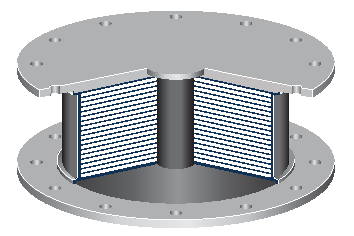
\includegraphics[scale=1]{E_IMAGENES/2_Capitulo2/Cap2_Imagen1a.pdf}
	\caption{\centering\footnotesize Aislador eslastomérico LRB. Adaptado de \citet{Bridgestone2015}}
  	\label{Cap2_Figura1a}
	\end{subfigure}
	\hfill
	\begin{subfigure}[b]{0.45\textwidth}
  	\centering
  	% include second image
  	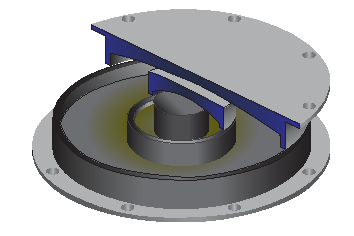
\includegraphics[scale=1]{E_IMAGENES/2_Capitulo2/Cap2_Imagen1b.pdf} 
  	\caption{\centering\footnotesize Aislador friccionante TFPB. Adaptado de \citet{Fenz2008}}
  	\label{Cap2_Figura1b}
	\end{subfigure}
	\caption[Dispositivos de aislamiento sísmico]{\centering\footnotesize Dispositivos de aislamiento sísmico}
	\label{Cap2_Figura1}
	\end{figure}
	
	\subsection{Disipadores de Fluido Viscoso}
Son dispositivos que incrementan el amortiguamiento de la estructura sin incrementar la rigidez y cuyo funcionamiento depende fundamentalmente de la velocidad relativa de sus extremos. Los DFV están compuestos por un pistón de acero inoxidable, con cabezal de bronce y un acumulador, que se encuentran alojados dentro en un cilindro metálico lleno con un fluido de alta viscosidad. La cabeza del pistón tiene orificios que están diseñados con una serie de formas especiales para alterar las características de flujo con la velocidad del fluido, disipando de esta manera energía en forma de calor. La construcción mecánica y las propiedades del orificio se pueden variar para obtener las propiedades amortiguadoras deseadas \citep{Constantinou1993}.

	\begin{figure}[!h]
	\centering
		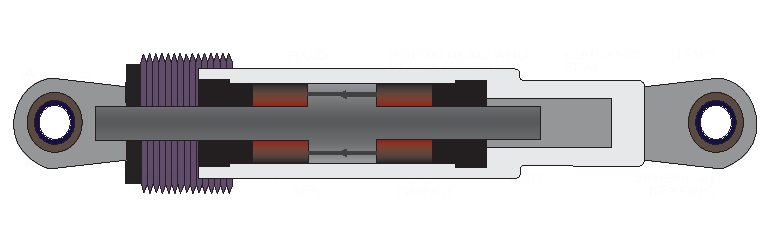
\includegraphics[scale=1]{E_IMAGENES/2_Capitulo2/Cap2_Imagen2.pdf}
	\caption[Disipador de fluido viscoso]{\centering\footnotesize Disipador de fluido viscoso.  Adaptado de \shortcites{Taylor2019}\citet{Taylor2019}}
	\label{Cap2_Figura2}
	\end{figure}
	
	
	
	


	\section{SEGUNDO TEMA}

En esta sección se revisan modelos matemáticos capaces de describir de forma analítica una amplia gama de comportamientos inelásticos complejos presentes en muchos sistemas y materiales.

	\subsection{Modelo Histerético de Bouc-Wen} \label{subsection:MHBW}
	
Es un modelo que se usa para predecir el comportamiento dinámico no lineal de aisladores sísmicos, así como de disipadores histeréticos. El modelo de Bouc-Wen necesita cuatro parámetros de entrada, los cuales son: la rigidez elástica, la rigidez postfluencia, la fuerza característica y un parámetro adimensional que controla la forma del lazo histerético.

De acuerdo con \citet{Charalampakis2010} la fuerza en el tiempo \textit{t} del modelo histerético de Bouc-Wen se evalúa en función del desplazamiento de la siguiente manera:
\begin{gather}
F(t)=\alpha \frac{F_{y}}{D_{y}}u(t)+(1-\alpha)F_{y}z(t)				\label{BoucWen1} \\
\begin{aligned}
\dot{z}(t)=\left[1-\left|z(t)\right |^{\eta}sgn(\dot{u}(t)z(t))\right]\frac{\dot{u}(t)}{D_{y}}&,&\hspace{1em}& z(0)=0 \\
\end{aligned}		\label{BoucWen2}
\end{gather}

	\begin{figure}[!h]
	\centering
		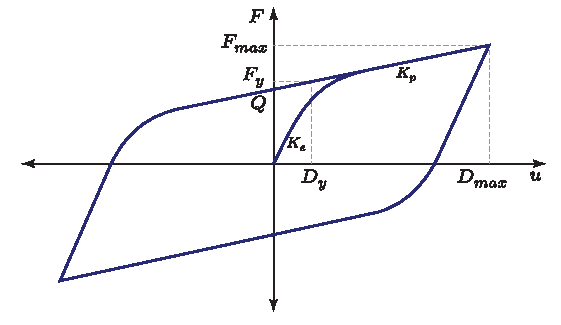
\includegraphics[scale=1]{E_IMAGENES/2_Capitulo2/Cap2_Imagen6.pdf}
		%\vspace{-3 mm}
	\caption[Modelo histerético de Bouc-Wen]{\centering\footnotesize Modelo histerético de Bouc-Wen. Adaptado de \citet{Charalampakis2010}}
	\label{Cap2_Figura6}
	\end{figure}

En la \autoref{Cap2_Figura6} y en las ecuaciones \ref{BoucWen1} y \ref{BoucWen2} se muestran los parámetros necesarios para definir un ciclo histerético con comportamiento de Bouc-Wen.

Donde:

%Inicar tabla explicando cada Parámetro
\begin{tabular}{L{0.5 cm}p{0.025 cm}p{11.5 cm}}
  $K_{e}$ & : & Rigidez elástica \\
  $K_{p}$ & : & Rigidez postfluencia \\
  $Q$     & : & Fuerza característica \\
  $D_{y}$ & : & Desplazamiento de fluencia \\
  $F_{y}$ & : & Fuerza de fluencia \\
  $\alpha$ & : & Razón entre la rigidez postfluencia y la rigidez elástica  \\
  $\eta$ & : & Parámetro adimensional que controla la forma del lazo histerético \\
 \end{tabular}\\

	
 
 
	
	\section{TERCER TEMA}
 
	\subsection{Modelo de Masas Concentradas}
	
\begin{definition}[Modelo de Masas Concentradas]
	Es un modelo físico discreto conformado por una serie de masas interconectadas por resortes sin peso (sistema de acoplamiento cercano). Este modelo puede describir adecuadamente el comportamiento de edificaciones con un sistemas estructural basado en pórticos con vigas muy rígidas y donde las deformaciones axiales de las columnas se desprecian.
\end{definition}

		\subsubsection{Matrices de Masa y Rigidez}

\begin{definition}[Matrices de Masa y Rigidez]
	Para un modelo discreto de masas concentradas de $n$ GDL, la matriz de masas $\mathbfit{M}$ es diagonal, con la masa $i_{\acute{e}sima}$, $m_{i}$, como el elemento diagonal $i_{\acute{e}simo}$.
	
	\begin{equation}\label{Eq18}
		M=\begin{bmatrix}
			m_{1} & 0 & 0 & \cdots & 0 & 0 \\ 
			0 & m_{2} & 0 & \cdots & 0 & 0\\ 
			0 & 0 & m_{3} & \cdots & 0 & 0\\ 
			\vdots & \vdots & \vdots &\ddots  &\vdots  &\vdots \\ 
			0 & 0 & 0 & \cdots & m_{n-1}& 0\\ 
			0 & 0 & 0 & \cdots & 0 & m_{n}
		\end{bmatrix}_{n\times n}
	\end{equation}
\end{definition}



		\subsubsection{Matriz de Amortiguamiento}

\begin{definition}[Matriz de Amortiguamiento]
	Usando el amortiguamiento de Rayleigh se puede construir una matriz de amortiguamiento que sea consisten con los datos experimentales \citep{Chopra2016}. Tal como se aprecia en la ecuación \ref{Eq21}, Rayleigh propone que la matriz de amortiguamiento sea una combinación lineal de la matriz de masa y la matriz de rigidez.
	\begin{equation}\label{Eq21}
		\mathbfit{C}=a_{0}\mathbfit{M}+a_{1}\mathbfit{K}
	\end{equation}
\end{definition}

	
	\section{CUARTO TEMA}

De acuerdo con la ASCE 7-16 y la norma E.031 cuando se realice un análisis tiempo historia para diseñar edificaciones que incorporen algún sistema de control pasivo se debe usar un mínimo de siete registros sísmico, los cuales deben estar escalados correctamente. Dado que el objetivo de la presente tesis no es realizar un diseño detallado sino más bien conocer la eficiencia de cada sistema de control pasivo en la reducción de la respuesta sísmica, se usaron solo tres registros.

	\subsection{Registros Sísmicos Ajustados}
	
A continuación se presentan los registros sísmicos usados en la presente tesis.
			
	\begin{figure}[h!]
	\centering
	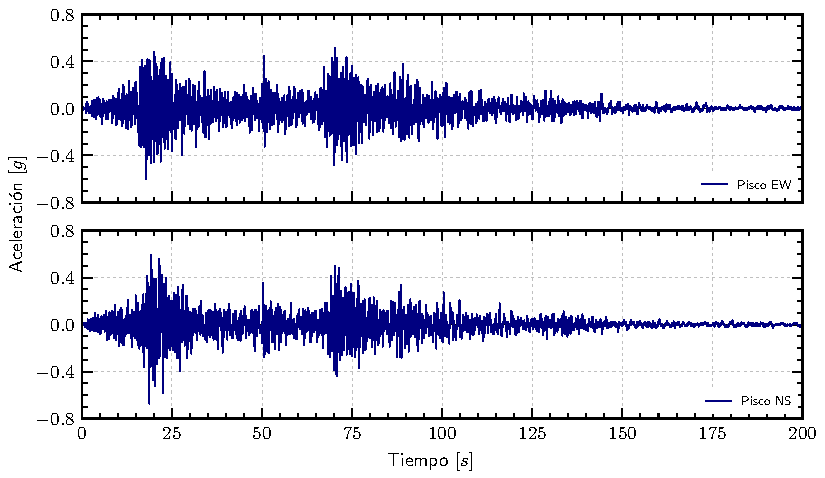
\includegraphics[scale=1]{E_IMAGENES/2_Capitulo2/Cap2_PiscoSc.pdf}
	\vspace{-8 mm}
	\caption[Acelerogramas espectrocompatibles - Pisco 2007]{\centering\footnotesize Acelerogramas espectrocompatibles - Pisco 2007.}
	\label{Cap2_Figura15}
	\end{figure}	
			

	


	
		
	% CAPÍTULO 3
	\chapter{NOMBRE DEL CAPÍTULO 3}
\markboth{CAPÍTULO \thechapter: NOMBRE DEL CAPÍTULO 3}{}

\lipsum [6]

	\input{2_CAPITULO3/Secciones/1_Primera Sección.tex}
	
	\input{2_CAPITULO3/Secciones/2_Segunda Sección.tex}
	
	\input{2_CAPITULO3/Secciones/3_Tercera Sección.tex}
	
	\input{2_CAPITULO3/Secciones/4_Cuarta Sección.tex}




		


		
	% CAPÍTULO 4
	\chapter[NOMBRE DEL CAPÍTULO 4]{NOMBRE DEL CAPÍTULO 4}
\markboth{CAPÍTULO \thechapter: NOMBRE DEL CAPÍTULO 4}{}

\lipsum[10]

	\input{2_CAPITULO4/Secciones/1_Primera Sección.tex}
	
	\input{2_CAPITULO4/Secciones/2_Segunda Sección.tex}
	




		

		
	
	%Parte FINAL DE LA TESIS
	
	\backmatter

	% CONCLUSIONES Y RECOMENDACIONES
	\cleardoublepage\phantomsection\addcontentsline{toc}{chapter}{\bf CONCLUSIONES}
\chapter*{\centerline {CONCLUSIONES}}
\markboth{CONCLUSIONES}{}
%--
\begin{enumerate}

\item Nam dui ligula, fringilla a, euismod sodales, sollicitudin vel, wisi.  Morbiauctor lorem non justo. Nam lacus libero, pretium at, lobortis vitae, ultricies et,tellus. Donec aliquet, tortor sed accumsan bibendum, erat ligula aliquet magna,vitae ornare odio metus a mi.

\item Nam dui ligula, fringilla a, euismod sodales, sollicitudin vel, wisi.  Morbiauctor lorem non justo. Nam lacus libero, pretium at, lobortis vitae, ultricies et,tellus. Donec aliquet, tortor sed accumsan bibendum, erat ligula aliquet magna,vitae ornare odio metus a mi.

\item Nam dui ligula, fringilla a, euismod sodales, sollicitudin vel, wisi.  Morbiauctor lorem non justo. Nam lacus libero, pretium at, lobortis vitae, ultricies et,tellus. Donec aliquet, tortor sed accumsan bibendum, erat ligula aliquet magna,vitae ornare odio metus a mi.


\end{enumerate}

	\cleardoublepage\phantomsection\addcontentsline{toc}{chapter}{\bf RECOMENDACIONES}
\chapter*{\centerline {RECOMENDACIONES}}
\markboth{RECOMENDACIONES}{}
%
\begin{enumerate}
\item Nam dui ligula, fringilla a, euismod sodales, sollicitudin vel, wisi.  Morbiauctor lorem non justo. Nam lacus libero, pretium at, lobortis vitae, ultricies et,tellus. Donec aliquet, tortor sed accumsan bibendum, erat ligula aliquet magna,vitae ornare odio metus a mi.

\item Nam dui ligula, fringilla a, euismod sodales, sollicitudin vel, wisi.  Morbiauctor lorem non justo. Nam lacus libero, pretium at, lobortis vitae, ultricies et,tellus. Donec aliquet, tortor sed accumsan bibendum, erat ligula aliquet magna,vitae ornare odio metus a mi.

\item Nam dui ligula, fringilla a, euismod sodales, sollicitudin vel, wisi.  Morbiauctor lorem non justo. Nam lacus libero, pretium at, lobortis vitae, ultricies et,tellus. Donec aliquet, tortor sed accumsan bibendum, erat ligula aliquet magna,vitae ornare odio metus a mi.


\end{enumerate}
	
	% REFERENCIAS BIBLIOGRÁFICAS
	\cleardoublepage\phantomsection\addcontentsline{toc}{chapter}{\bf REFERENCIAS BIBLIOGRÁFICAS}
\begingroup
\titleformat*{\chapter}{\normalfont\bfseries\normalsize\centering}
\bibliography{3_2_BIBLIOGRAFIA/library}
\endgroup


	
	% ANEXOS	
	\cleardoublepage\phantomsection\addcontentsline{toc}{chapter}{\bf ANEXOS}
\chapter*{\centerline {ANEXOS}}
\markboth{ANEXOS}{}
%---

% Definir númeración y citación para Listing 

\renewcommand{\lstlistingname}{ \footnotesize Código A \hspace{-1.75mm}}% Cambiar el nombre a Algoritmo
\renewcommand*{\thelstlisting}{.\arabic{lstlisting}} 
\def\lstlistingautorefname{Código A\hspace{-0.75mm}}

% Redefinir númeración y citación para Figuras
\renewcommand\thefigure{.\arabic{figure}}  
\setcounter{figure}{0} 
\renewcommand\figurename{\footnotesize FIGURA B \hspace{-1.6mm}}
\def\figureautorefname{Figura B \hspace{-2mm}}


	\section*{ANEXO A: CÓDIGOS EN PYTHON}
\phantomsection
\addcontentsline{toc}{section}{ANEXO A: CÓDIGOS EN PYTHON}
A continuación se presentan los códigos desarrollados en \textit{Python}. En este sentido, el \autoref{Algoritmo1} muestra el algoritmo usado para edificaciones con aislamiento de base con comportamiento bilineal. El \autoref{Algoritmo2} muestra las funciones usadas por los algoritmos anteriormente mencionados.

\vspace*{2mm}


	\subsection*{Respuesta Sísmica de una Edificación con AS}
%\phantomsubsection
\addcontentsline{toc}{subsection}{Respuesta Sísmica de una Edificación con AS}

\begin{MyFont}
\begin{adjustwidth}{4.8mm}{}
\begin{lstlisting}[language=Python, caption= {\footnotesize Edificación con aislamiento sísmico bilineal}, mathescape=true,label={Algoritmo1}]
# REPUESTA SÍSMICA DE UNA EDIFICACIÓN DE n NIVELES CON AS
import Funciones_KS as fun
import numpy as np
from scipy  import linalg as LA
import copy

# PROPIEDADES DINÁMICAS
# Parámetros dinámicos de la Superestructura
n=3                 # N° de Pisos
gdl=n+1             # GDL = N° de Pisos+1
Tnf=0.3             # Periodo base fija, [s]
$\xi$=5           			 # Amortiguamiento, [%]
$\lambda$=(gdl-1)/gdl 			 # Relación de masas

# Parámetros dinámicos de la interfaz de aislamiento
r=0.1               # Razón de rigideces Kp/Ke
Q=105          		  # Fuerza característica normalizada, [cm/s^2]
K2=30         		  # Rigidez postfluencia normalizada, [1/s^2]

# LECTURA DEL REGISTRO SÍSMICO
ug=np.genfromtxt("./Sismo_Lima66NS.txt")  #[cm/s^2]
$\Delta$t=0.002; N=len(ug)
t=[i*$\Delta$t for i in range(N)]

\end{lstlisting}
\end{adjustwidth}
\end{MyFont}

	
	\subsection*{Funciones}
%\phantomsubsection
\addcontentsline{toc}{subsection}{Funciones}

\begin{MyFont}
\begin{adjustwidth}{4.8mm}{}
\begin{lstlisting}[language=Python, caption={\footnotesize Funciones-KS}, mathescape=true,label={Algoritmo2}]
import numpy as np
from scipy  import linalg as LA
import copy

# FUNCIÓN EIGEN
def eigen(Tsf=1,n=5):
    Z=np.identity(n); ke=(4*n/Tsf)**2; k=np.zeros(n)
    for i in range(n):
        if i==0:
            k[i]=2*ke
        else:
            k[i]=ke
    K=tridiag(k,n); M=np.identity(n)
    vp,$\varphi$p=LA.eigh(K,M); $\varphi$p=$\varphi$p.T; FP=[]; MP=[] 
    for i in range(n):
        FP.append(sum($\varphi$p[i].T@M))
    for i in range(n):
        MP.append((sum($\varphi$p[i].T@M))**2)
    T=2*np.pi/(vp)**0.5; MMP=MP/sum(MP)
    return T,$\varphi$p,FP,MMP

\end{lstlisting}
\end{adjustwidth}
\end{MyFont}

	\newpage

	\section*{ANEXO B: HISTÉRESIS DE LOS DISPOSITIVOS DE CONTROL}
\phantomsection
\addcontentsline{toc}{section}{ANEXO B: HISTÉRESIS DE LOS DISPOSITIVOS DE CONTROL}

\lipsum[10]

	\subsection*{Edificio Principal del Aeropuerto Jorge Chavez}
%\phantomsubsection
\addcontentsline{toc}{subsection}{Edificio Principal del Aeropuerto Jorge Chavez}

La \autoref{Anexo_1} muestra las histéresis de uno de los dos los DFV instalados en el eje 5-5 del primer nivel del edificio pincipal del aeropuerto Jorge Chavez. Asimismo, la \autoref{Anexo_2} presenta la histéresis de uno de los tres DH-SLB colocado en el eje 5-5 del primer nivel de la misma edificación.


	\begin{figure}[!h]
	\centering
	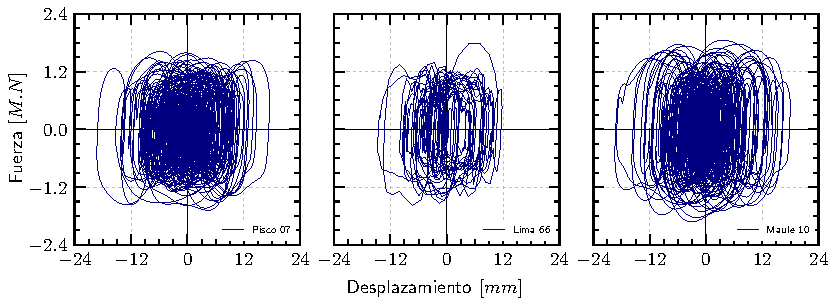
\includegraphics[scale=1]{E_IMAGENES/3_Anexos/Anexo_1.pdf}
	\vspace{-8 mm}
	\caption[]{\centering\footnotesize Histéresis del DFV del edificio del aeropuerto Jorge Chavez.}
	\label{Anexo_1}
	\end{figure}	


	\begin{figure}[!h]
	\centering
	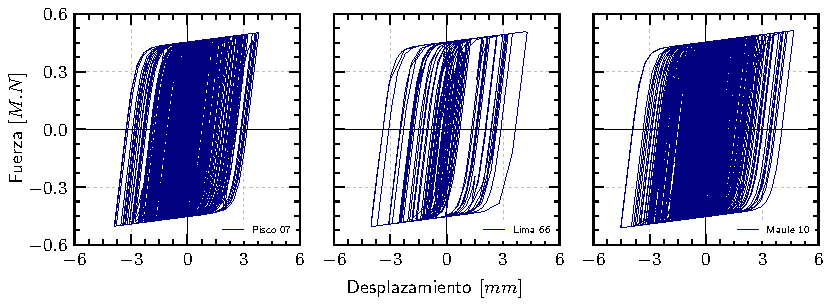
\includegraphics[scale=1]{E_IMAGENES/3_Anexos/Anexo_2.pdf}
	\vspace{-8 mm}
	\caption[]{\centering\footnotesize Histéresis del DH-SLB del edificio del aeropuerto Jorge Chavez.}
	\label{Anexo_2}
	\end{figure}	





	
\end{document}
